\documentclass{article}[letterpaper, 11pt]
\usepackage{geometry}
\geometry{left=0.75in,top=0.75in,bottom = 0.75in,right=0.75in}
\usepackage[utf8]{inputenc}
\usepackage{amsmath}
\usepackage{bbm}
\usepackage{amssymb}
\usepackage{enumitem}

\usepackage{lastpage}
\usepackage{fancyhdr}

\usepackage{svg}
\usepackage{graphicx}
\graphicspath{ {images/} }

\usepackage[parfill]{parskip}

\usepackage{color}   %May be necessary if you want to color links
\usepackage{hyperref}
\hypersetup{
    colorlinks=true, %set true if you want colored links
    linktoc=all,     %set to all if you want both sections and subsections linked
    linkcolor=black,  %choose some color if you want links to stand out
}

%Style :
\pagestyle{fancy}
\renewcommand{\thepage}{}
%commancer le compte des pages après
\setlength{\headsep}{14.5pt}

%Style nouveau chapitre
\fancyhf{}
\fancyhead[L]{\small INF8770 --- Technologies multimédias}
\fancyhead[C]{\small TP2 --- Compression transformée KL}
\fancyhead[R]{\small Page \thepage\hspace{1pt} sur~\pageref{LastPage}}
\fancyfoot[L]{\scriptsize Polytechnique Montréal}
\fancyfoot[C]{\scriptsize Matthieu Basset, Hiver 2024}
\fancyfoot[R]{\scriptsize Département de GIGL}
\renewcommand{\headrulewidth}{0.5pt}
\renewcommand{\footrulewidth}{0.2pt}

\title{
    
\includegraphics[scale=0.8]{poly-logo.pdf}\\\vspace*{50pt}
    \huge\textbf{INF8770}\\
    \textbf{Technologies Multimédias}\\
    Travail pratique \#2\\
    Compression d'images avec la transformée \\Karhunen-Loève\\
}

\author{\Large Matthieu Basset --- 2225981}
\date{\huge Février 2024}
\begin{document}

\thispagestyle{empty}
\maketitle

\newpage

\renewcommand{\thepage}{\arabic{page}}
\pagestyle{fancy}
\renewcommand{\contentsname}{Table des matières}
\setcounter{page}{1}

\tableofcontents


\newpage
\section{Question 1}
La transformée KL vise à passer une image dans la base des vecteurs propres de la matrice de covariance associée à la valeur de ses pixels après que ces derniers aient été centrés. En d'autres termes, cette opération permet de transformer les données afin de travailler sur les composantes contribuant le plus à la variance de l'image. Cette représentation est très utile, en effet travailler dans cet espace permet de plus facilement réduire la quantité de détails liée à des données apporant moins d'informations à l'image d'origine.

Pour effectuer cette transformation, on commence par centrer les données en leur soustrayant leur moyenne, cela permet d'éviter les biais lors de la recherche de vecteurs propres. On calcule ensuite la matrice de covariance de la liste de vecteurs obtenue. On peut ensuite obtenir ses vecteurs propres, ce qui permet de passer les données dans l'espace lié à ces vecteurs. On peut effectuer différentes opérations sur les données tant qu'elle sont dans cet espace. On peut ensuite retrouver l'espace de base en calulant la matrice pseudo inverse liée à la matrice de vecteurs propres et ajouter la moyenne soustraite auparavant. On retrouve ainsi l'image dans un espace similaire à celui d'origine.

Cette transformée se distingue des transformées DCT et en ondelettes par les éléments sur lesquels elle opère. Ces deux dernières décomposent le signal en somme de signaux periodiques, là où la transformée KL cherche les axes de plus grande variance dans l'image

\newpage
\section{Question 2}

L'implémentation du TP est réalisée en python via un notebook. On trouve les résultats suivants pour la compression, utilisant des niveaux $8/8/8$, $8/8/4$, $8/8/0$ et $8/6/4$, et en utilisant l'espace colorimétrique RGB ou YUV:\@

\begin{figure}[h]
    \centering
    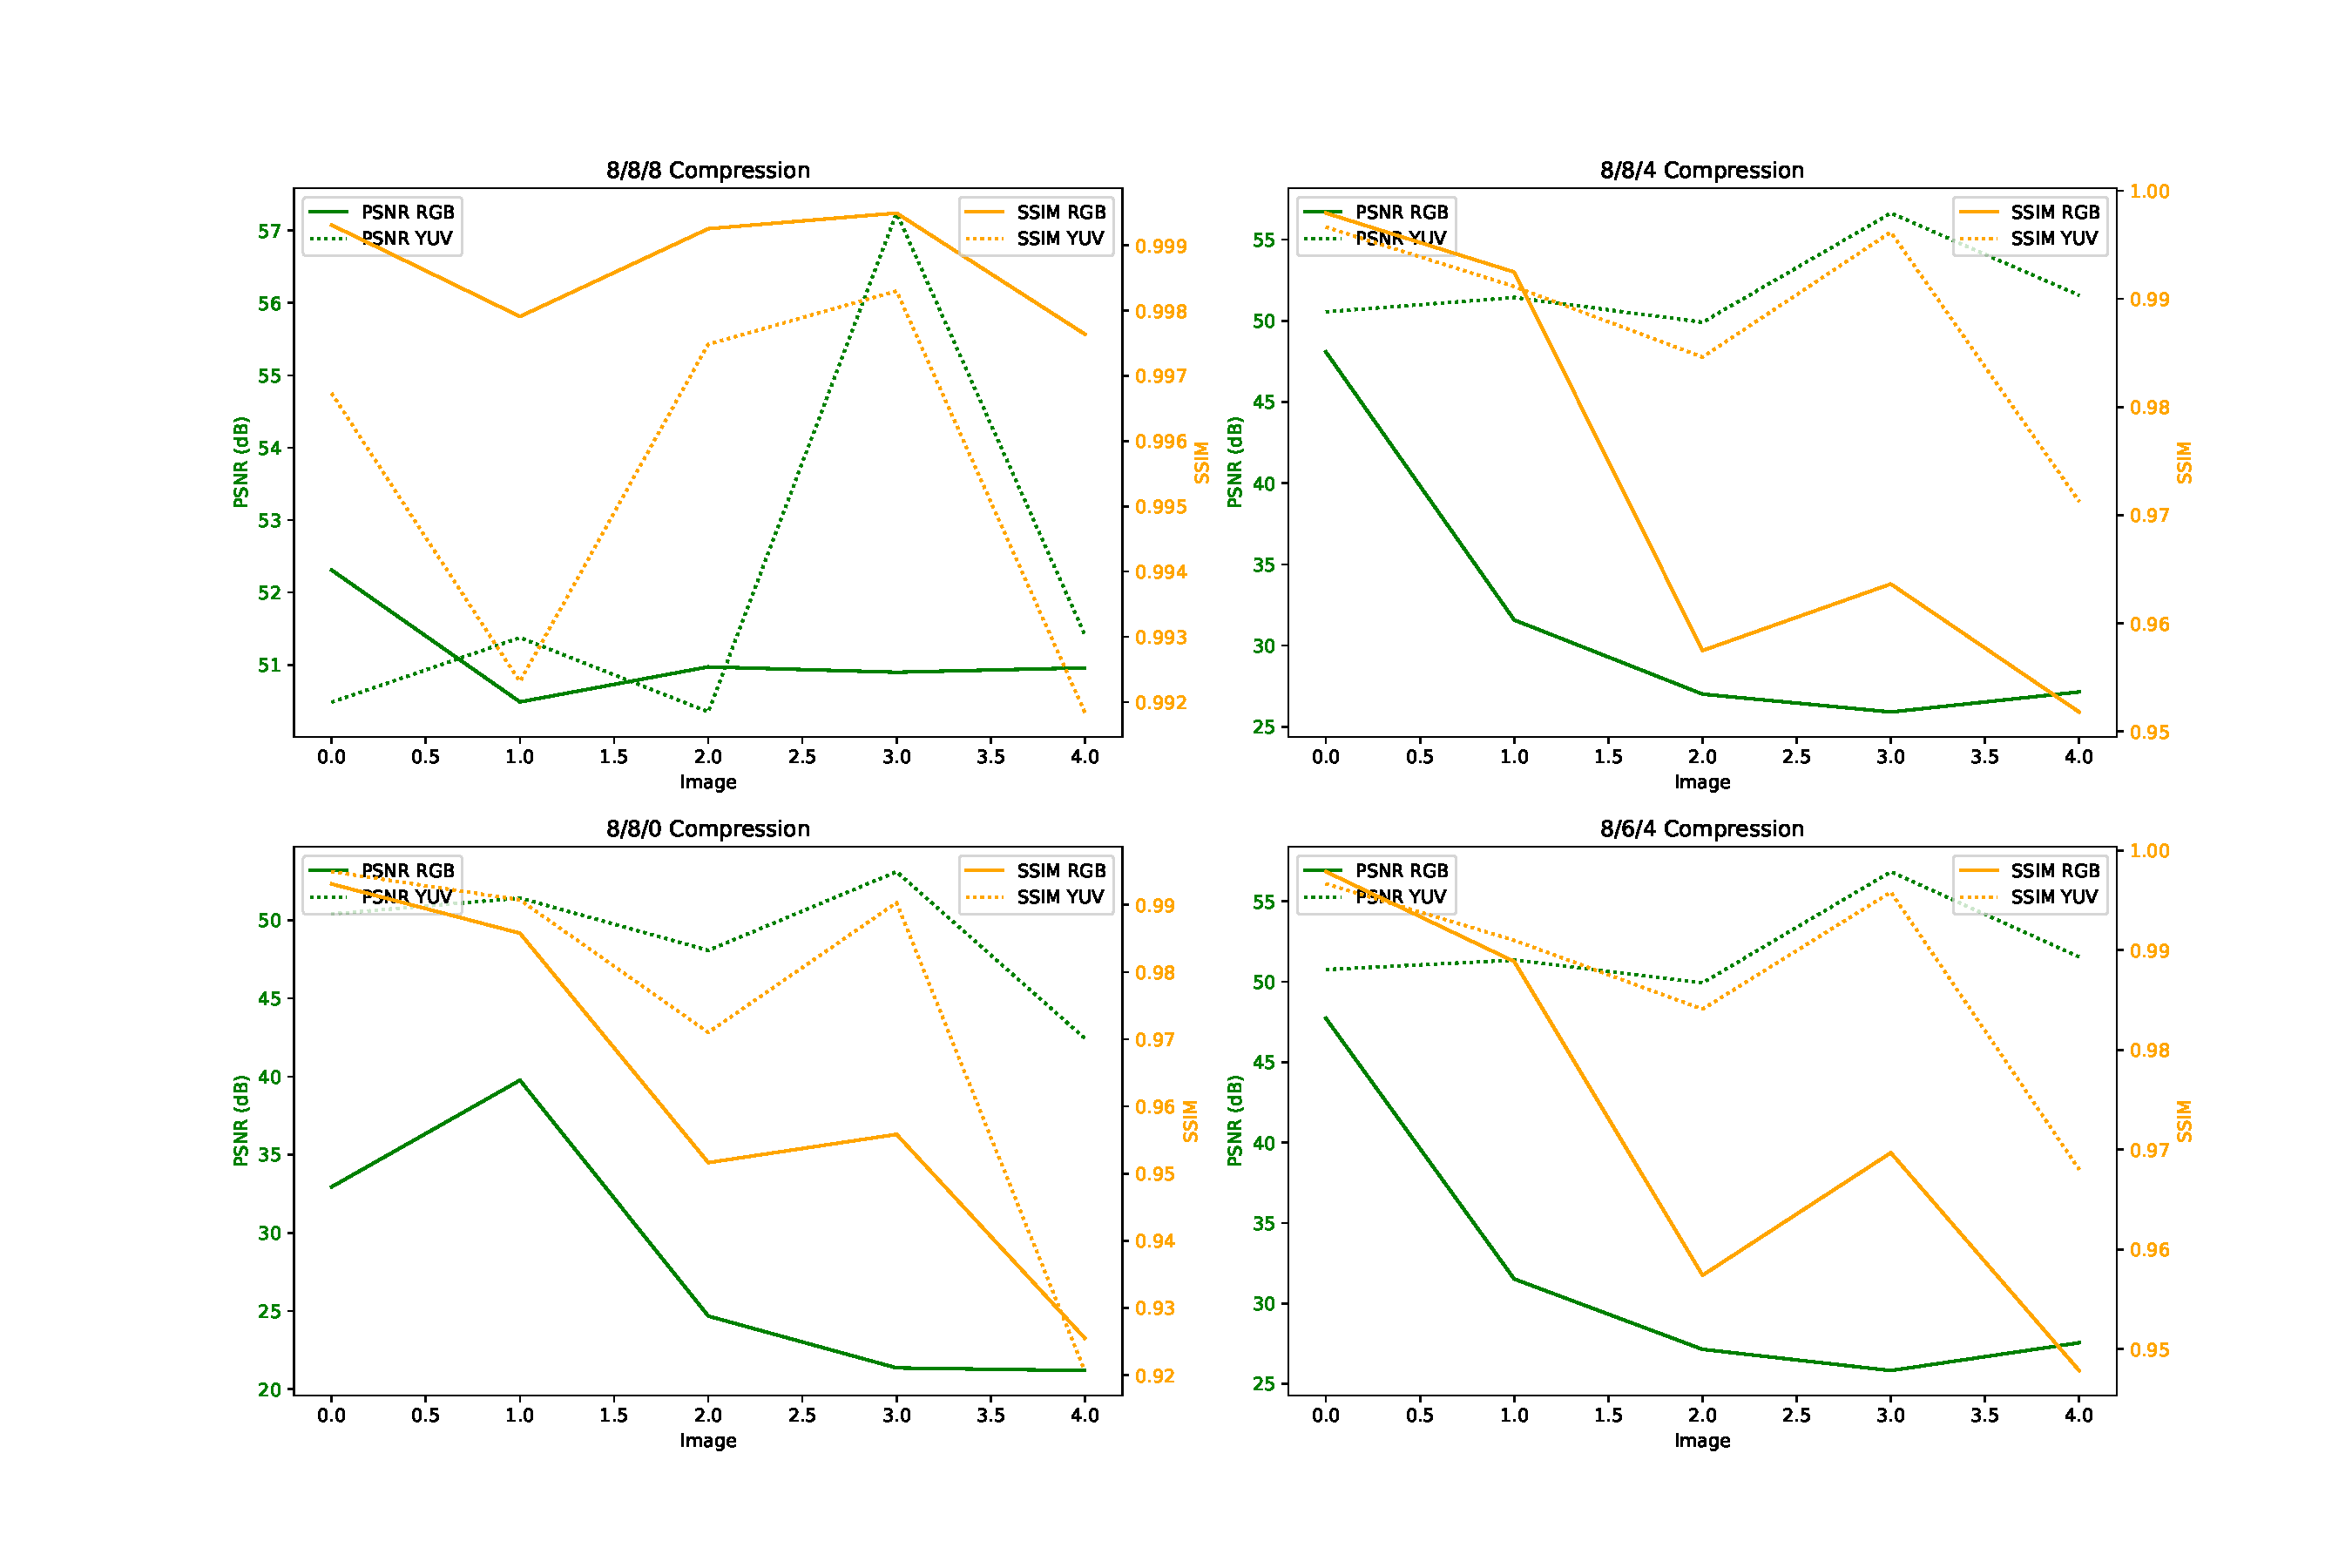
\includegraphics[scale=0.35]{all.pdf}
    \caption{Résultats pour chaque image}
\end{figure}
\newpage
\section{Question 3}
Lorsque l'on s'intéresse à la métrique de qualité couplé au taux de compression, ce sont les quantifications $8/8/0$ qui offrent le compromis le plus satisfaisant. Certes la qualité de l'image est dégradée de manière visible, mais la compression offerte compense cette perte. On notera que par opposition aux autres méthodes, une quantification aggressive sur une image dans l'espace de la transformée KL donnera des artefacts plus violents visuellement.

Pour ce qui est de l'espace de couleur le plus approprié, pour la métrique PSNR, l'espace YUV offre de meilleurs résultats, pour la métrique SSIM, les résultats sont plus proches. Ces métriques étant basées sur la perception humaine, il est naturel que l'espace YUV donne de meilleurs résultats. En effet cet espace est également conçu de manière à discriminer les composantes de couleur pour la compression adaptée à l'œil humain.

Ainsi, on peut conclure que la combinaison maximisant le rapport qualité/compression est une quantifiaction $8/8/0$ utisée sur une image YUV.\@

\begin{figure}[h]
    \centering
    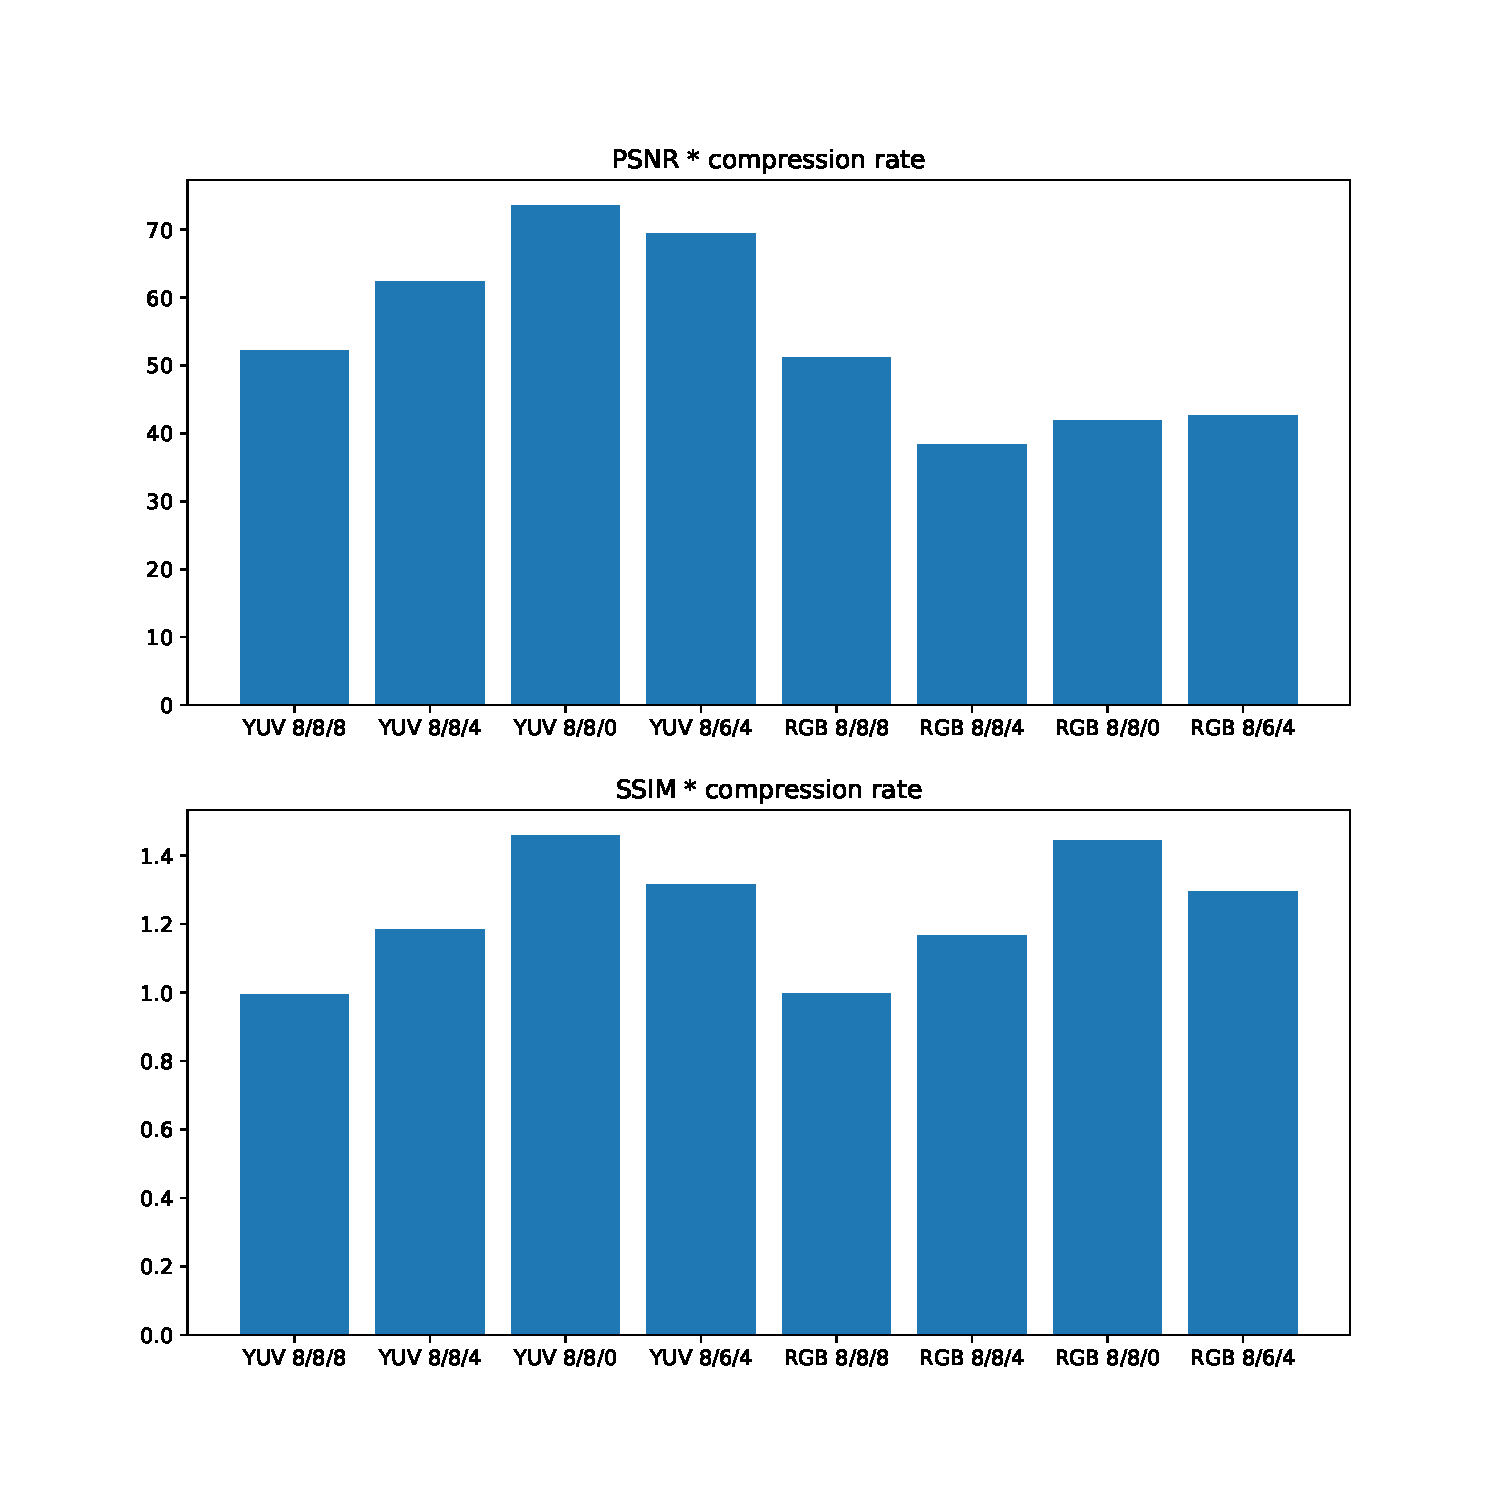
\includegraphics[scale=0.45]{averages.pdf}
    \caption{Résultats moyens qualité/compression pour chaque paramètre}
\end{figure}

\newpage
\section{Question 4}
D'un point de vue implémentation, il suffit de découper l'algorithme précédent et de remplacer les matrices de vecteurs propre par celles d'autres images.

On obtient les résultats suivants pour la compression d'une image $i$ en abscisse dans la base d'une image $j$ en ordonée.

Le taux de compression est de $33.3\%$ pour chaque image car les niveaux de quantification $8/8/0$ avaient été retenus à la question précédente.

\begin{figure}[h]
    \begin{minipage}[c]{.49\linewidth}
        \centering
        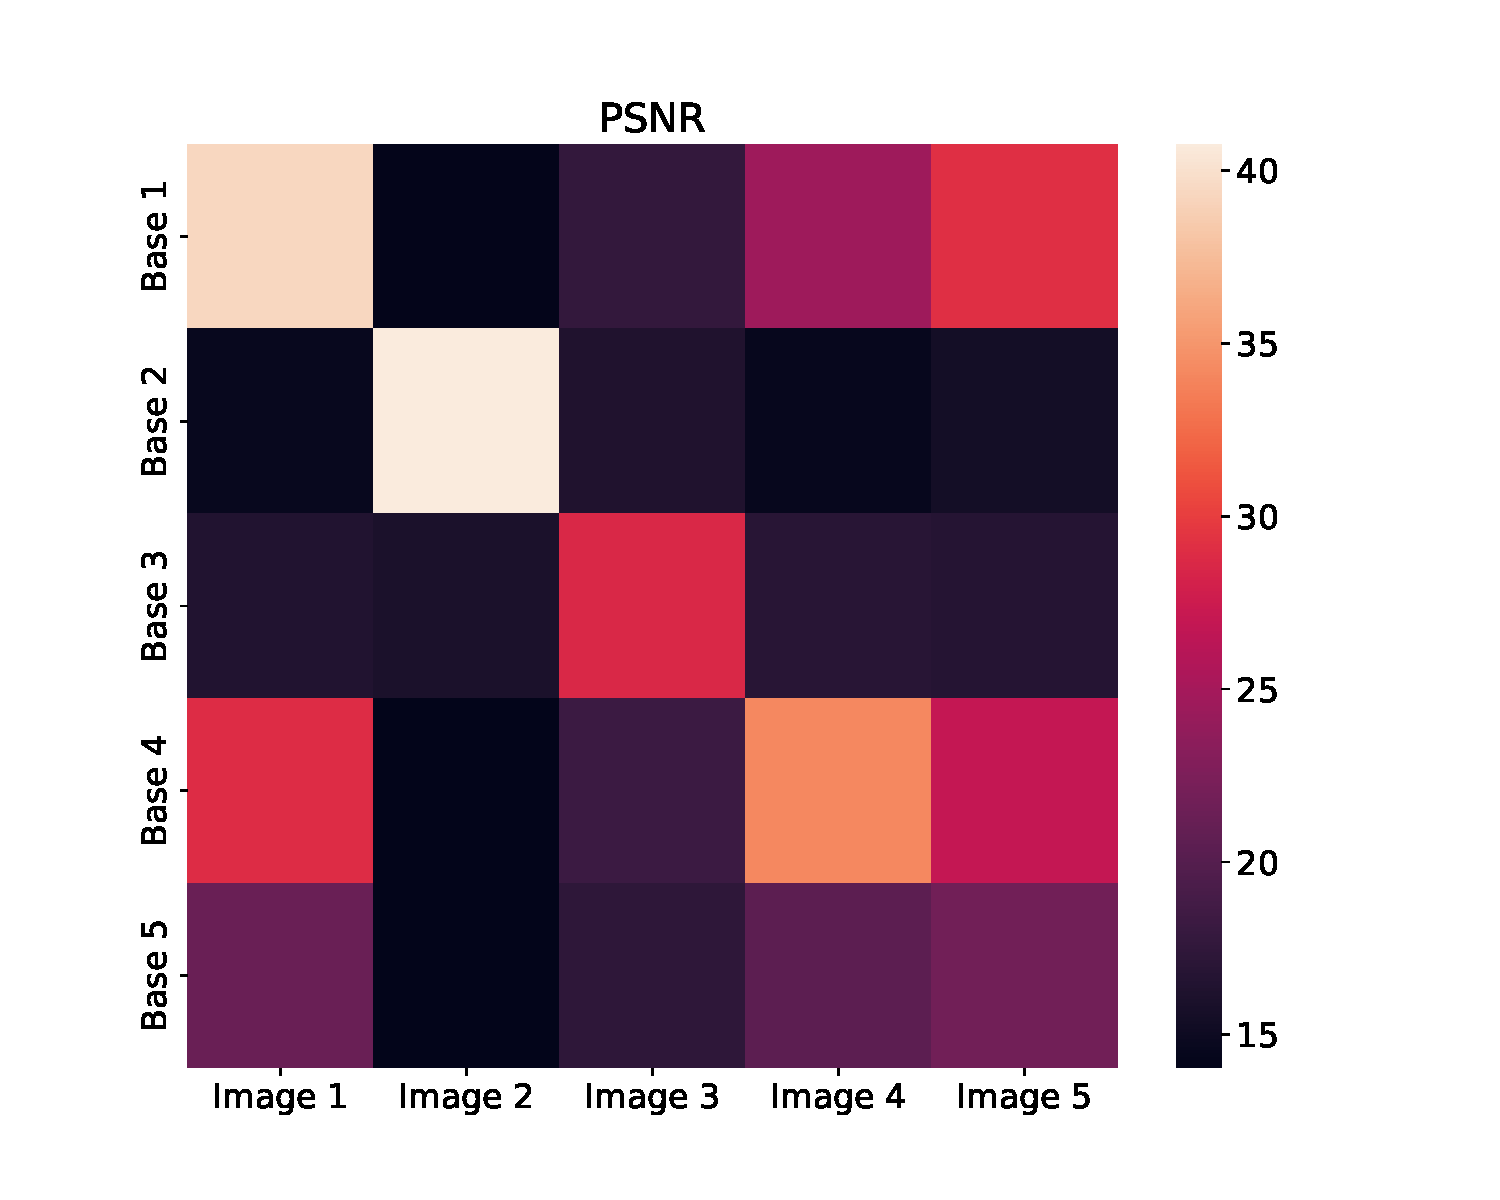
\includegraphics[scale = 0.25]{psnr.pdf}
    \end{minipage}
    \begin{minipage}[c]{.49\linewidth}
        \centering
        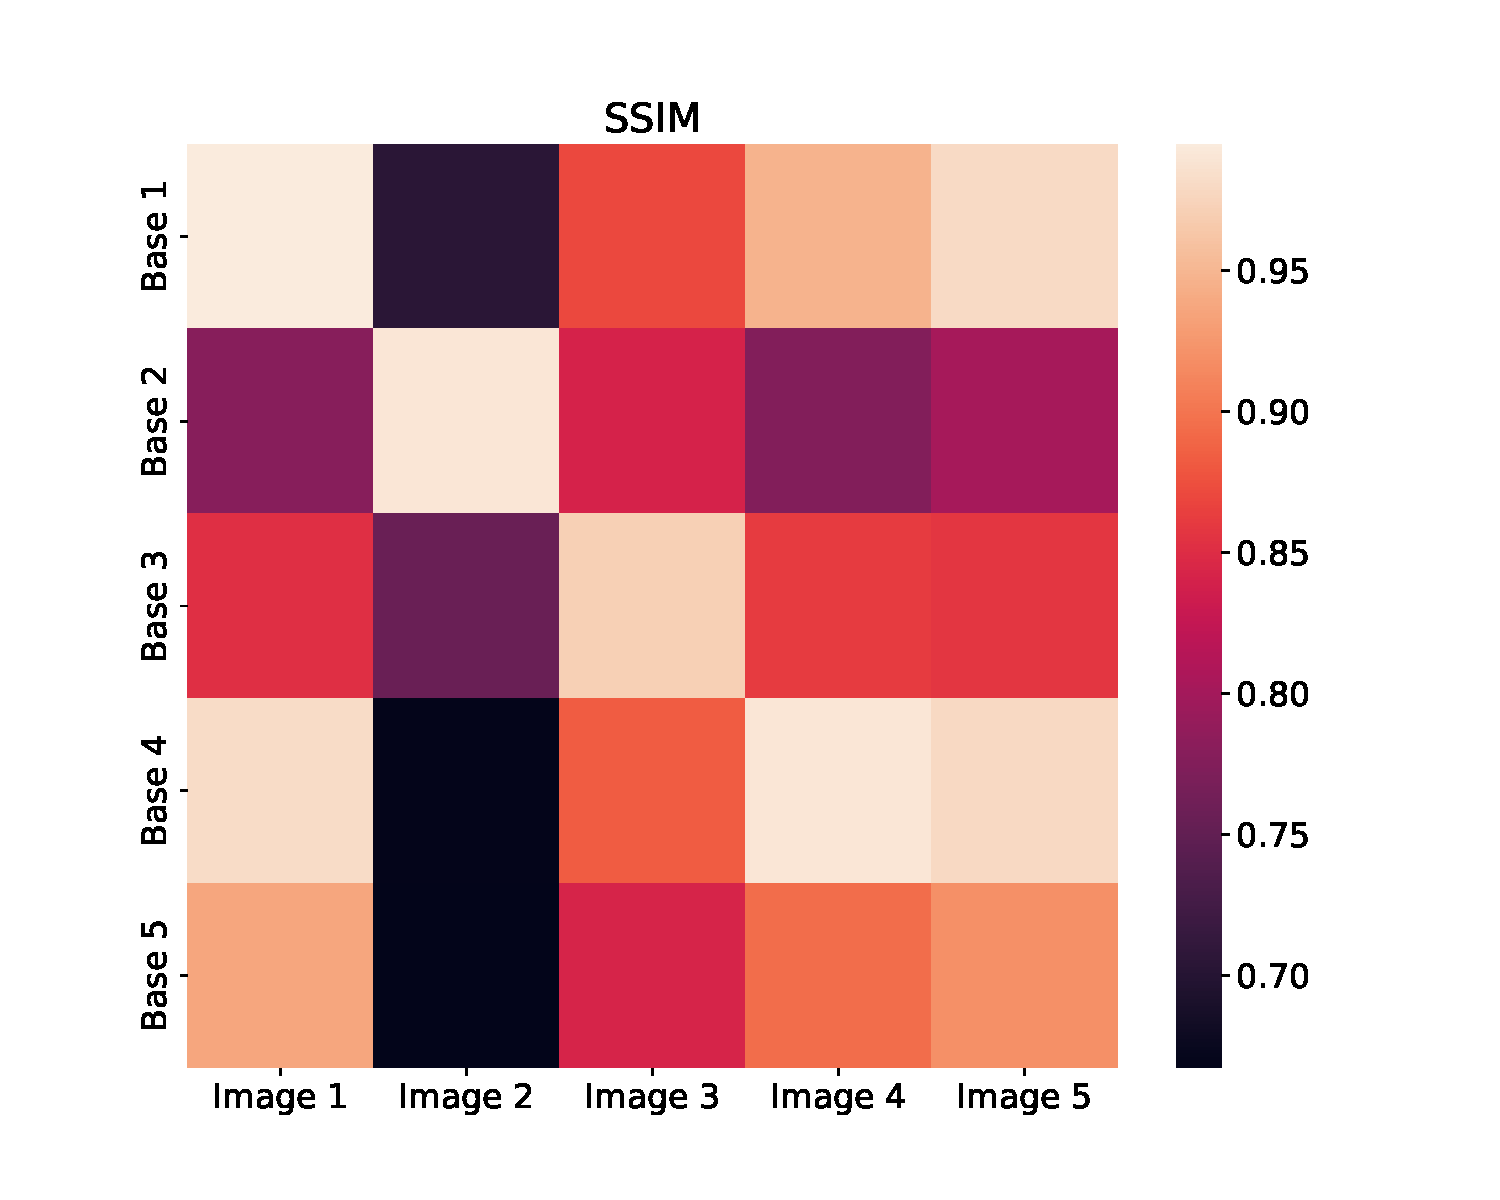
\includegraphics[scale = 0.25]{ssim.pdf}
    \end{minipage}
    \caption{Valeurs de PSNR et SSIM pour les images qunaitifiées dans d'autres bases.}
\end{figure}

\newpage
\section{Question 5}
On peut remarquer sans surprise que les résultats de qualité sont inférieurs sur les chaque image n'utilisant pas sa décomposition comme base pour la transformation. C'est d'ailleurs là une illustration d'un problème de la transformée KL, elle nécessite de calculer la base de vecteurs propre pour chaque image. Par opposition à DCT qui utilise une base standard de cosinus, on LZ77 que l'on peut uitiliser sur des dictionnaires pré-construits.

On remarquera cependant que certaines combinaisons donnent des résultats plutôt satisfaisant, les images 1 et 4 utilisées comme base donnent des résultats aceptables pour les mesures de SSIM (excepté pour l'image 2 qui donne des résultats médiocres pour chaque autre base utilisée, sûrement dû à sa structure particulière très unie).
\end{document}
